% !Mode:: "TeX:UTF-8
\documentclass[border=2pt]{standalone}

\usepackage{tikz}

\begin{document}

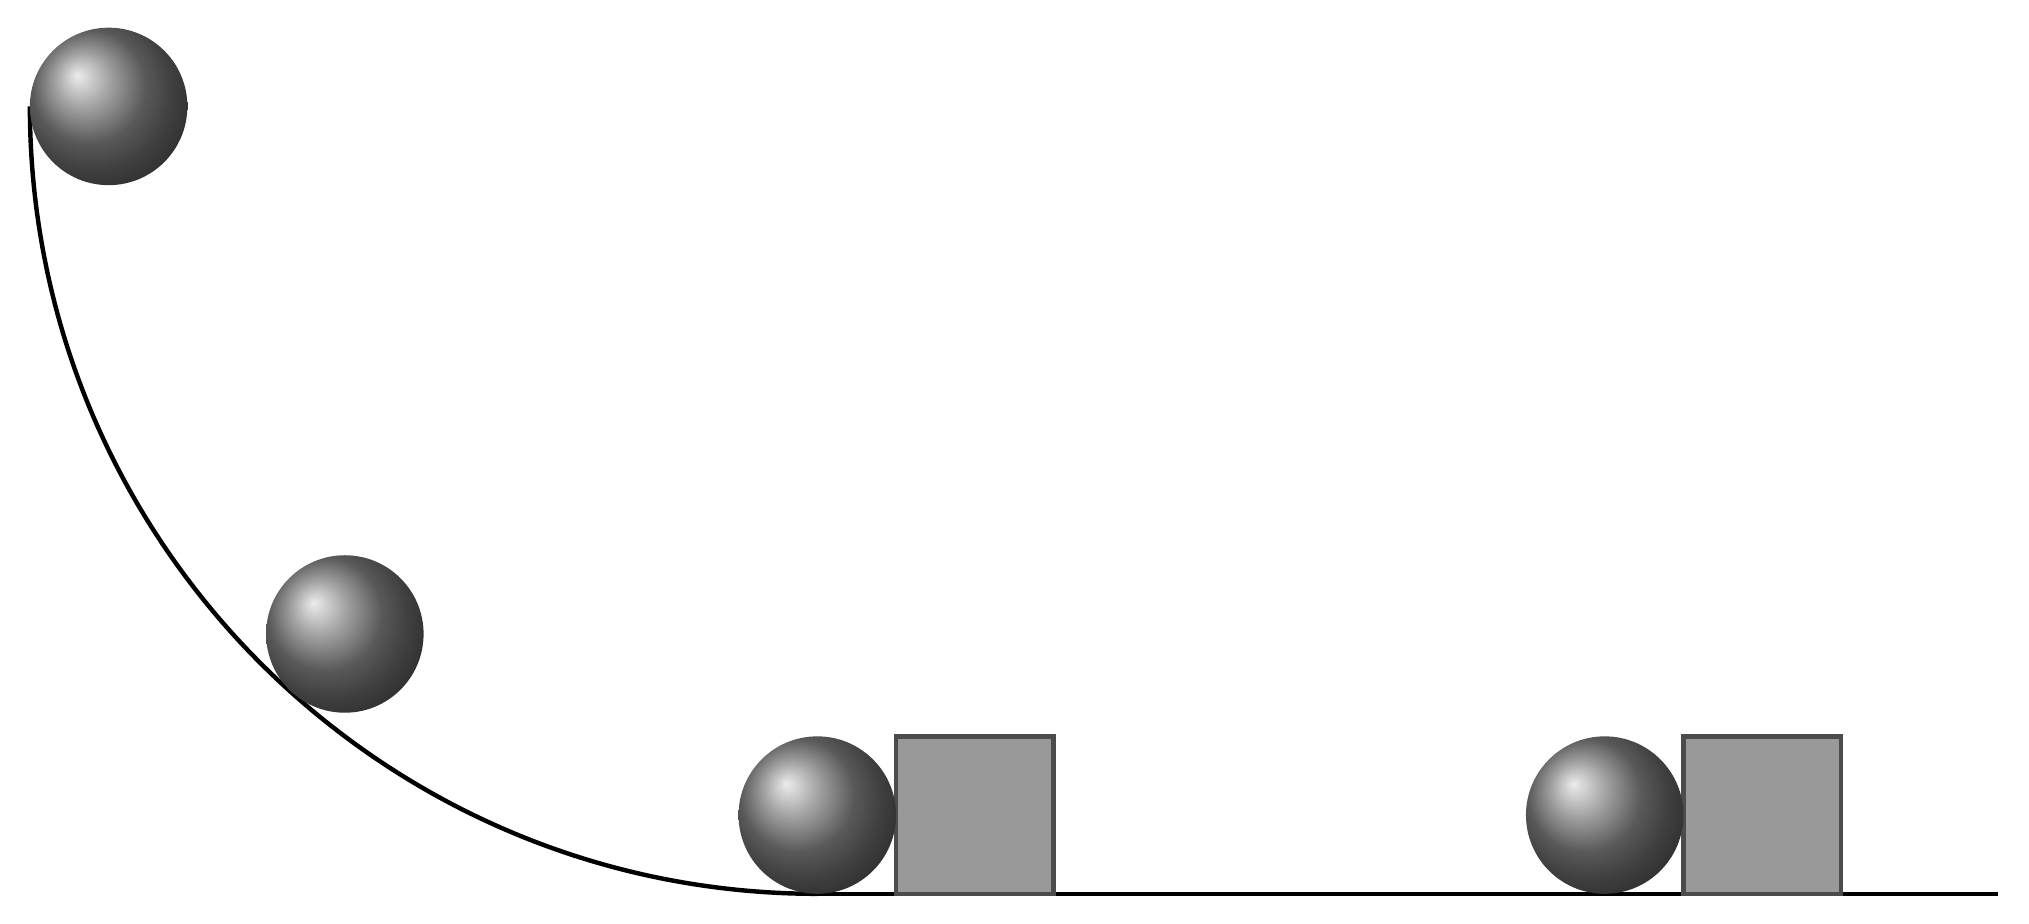
\begin{tikzpicture}
\newcommand{\rbox}[3][]{
\begin{scope}[#1]
\def\boxlen{#2}
\def\boxhei{#3}
%\draw[color=black!70,fill = black!40,ultra thick] (0,0) -- (\boxlen,0) -- (\boxlen,\boxlen) -- (0,\boxlen) --cycle;
\draw[color=black!70,fill = black!40,ultra thick] (0,0) rectangle (\boxlen,\boxhei);
\end{scope}}

\newcommand{\ball}[2][]{
\begin{scope}[#1]
\def\ballradius{#2}
\shade (0,0) circle  (\ballradius);
\end{scope}}




\draw[ultra thick] (0,0) arc (180:270:10cm);
\ball[ball color=gray,xshift=1cm]{1cm}


\draw[ultra thick] (10,-10) -- (25,-10);
\ball[ball color=gray,xshift=4cm,yshift=-6.7cm]{1cm}

\rbox[xshift=11cm,yshift=-10cm]{2cm}{2cm}
\ball[ball color=gray,xshift=10cm,yshift=-9cm]{1cm}

\begin{scope}[xshift=10cm]
\rbox[xshift=11cm,yshift=-10cm]{2cm}{2cm}
\ball[ball color=gray,xshift=10cm,yshift=-9cm]{1cm}
\end{scope}




\end{tikzpicture}

\end{document}